\documentclass[12pt]{article}
\usepackage[utf8]{inputenc}
\usepackage[french]{babel}
\usepackage{graphicx}
\usepackage{lipsum}
\usepackage{enumitem}
\usepackage{eurosym}
\usepackage[T1]{fontenc}

\usepackage[a4paper, total={14cm, 24cm}]{geometry}

\usepackage{fancyhdr}
\pagestyle{fancy}
\fancyhf{}
\fancyhead[LE,RO]{}
\fancyhead[RE,LO]{Mind the GAP}
\rfoot{\begin{center}\thepage\end{center}}
 

\setlength{\parskip}{2mm}

\title{Mind the GAP - Proposal}
\author{Toute l'équipe}
\date{Octobre 2016}

\begin{document}

\maketitle

\section{Introduction}
    Nous présentons ici notre projet intégré nommé GAP pour Génération Aléatoire de Plates-formes. Notre idée principale est, dans le cadre d'un jeu de plateforme, de mettre en place un générateur aléatoire de niveau qui permettrait de définir un environnement qui serait peu aisé à créer en tant qu'humain. Par exemple en reposant sur une physique déformée ou sur une augmentation du nombre de dimensions dans lesquelles le joueur peut évoluer. Ce projet cible les joueurs de jeux de plate-forme mais aussi les développeurs intéressés par la génération aléatoire de niveaux de jeu. \\
    Notre équipe dirigée par Rédouane Elghazi est composée de 10 membres:
    \begin{itemize}
        \renewcommand{\labelitemi}{$\bullet$}
        \item Guillaume Ambal
        \item Hugo Menet
        \item Loïs Paulin
        \item Nicolas Derumigny
        \item Pierre Mahmoud-Lamy
        \item Pierre-Etienne Polet
        \item Rédouane Elghazi
        \item Thomas Ragel
        \item Xavier Badin de Montjoye
        \item Yannis Gaziello
    \end{itemize}
    
\clearpage
\section{Description Détaillée}

    Nous avons décidé de séparer ce projet en deux parties distincte. Une première partie correspondant à la mise en place d'un générateur aléatoire de niveau. Et une seconde partie relevant de l'implémentation d'un jeu de plate-forme fonctionnel permettant d'explorer les niveaux générés. Nous devrons donc aussi définir l'interface entre ces deux parties.
    
    \subsection{Objectif du projet}
        
        Notre objectif global et de produire un jeu de plate-forme dont les niveaux sont générés aléatoirement, ce jeu doit être à la fois agréable à jouer et proposer de la difficulté de réalisation au joueur. L'objectif de la partie de mise en place du jeu est donc de définir un gameplay et une storyline de qualité, et de mettre tout cela en place dans un environnement visuellement attractif et offrant de multiples possibilités d'intéraction. Pour la partie de génération de niveau l'objectif est donc de générer un niveau qui exploite correctement le gameplay du jeu, qui puisse être fini et qui fournisse une bonne expérience de jeu au joueur. De plus, on souhaiterait que les niveaux générés soit suffisamment distinct pour éviter un sentiment de répétition.
        
    \subsection{Approche choisie}
    
        \subsubsection{Partie Jeu}
            Nous proposons de développer un jeu basé sur l'Unreal Engine 4. Nous utiliserons l'interface de blueprints proposée par le moteur afin de mettre rapidement en place une maquette fonctionnelle du jeu intégrant les éléments d'interaction principaux : le déplacement de l'avatar, le ramassage d'objets, activations de boutons, ...
            
            Le système de blueprints correspond à une interface graphique de développement, représentant sous forme de boîtes les concepts de la programmation événementielle. Nous utiliserons cet interface afin de définir notre physique de jeux, les éléments mobiles du décors, ainsi que toute interaction entre l'avatar du joueur et l'environnement de jeu. Les blueprints servirons aussi à mettre en place les interactions entre le joueur et le jeu. Nous prévoyons une interface manette avec possibilité alternative de jouer au clavier et à la souris.
            
            Nous allons à coté de cela construire une bibliothèque de maillages et de textures, en partie créés au sein de l'équipe et en partie piochés dans des bibliothèques libres de droits déjà existantes, afin d'offrir un ensemble d'éléments configurables qui pourront être utilisés dans la partie générateur.
            
            Notre jeu final prendra la forme d'un jeu de plate-forme en 3D à la première personne, potentiellement compatible VR, et joué à la manette ou au clavier. Un mode coopération est envisagé si les ressources temporelles sont disponibles.
            
        \subsubsection{Partie Générateur}
            L'idée de base du générateur est de placer chaque niveau dans un cube, ce cube contenant ainsi toutes les plate-formes permettant de relier le début et la fin du niveau, et permettant au joueur placé au début du niveau de contempler la totalité du niveau autour de lui. 

            Le niveau en lui même se compose d'un (ou plusieurs) chemin(s) reliant le début à la fin du niveau, composé de sous-niveaux vu comme des boîtes de tailles variables connectés entre elles. Le principe de la génération étant de ne pouvoir passer d'un sous-niveau à un autre seulement si les deux sous-niveaux sont reliés dans la conception du chemin. Par exemple si on a un unique chemin, chacun des sous-niveaux ne sera relié qu'a deux autres. Pour obtenir une impression d'ouverture du niveau, il faut le moins possible cloisonner (avec des murs par exemple) les sous-niveaux. On va donc construire notre chemin en faisant attention à ne pas pouvoir passer entre deux boîtes qui ne sont pas reliés. Ce qui correspond par exemple a suffisamment éloigner verticalement deux sous-niveaux pour que tomber de l'un vers l'autre soit rendu impossible par des dégâts de chute. On arrangera les sous-niveaux en prenant une zone autour d'eux, que l'on nomme zone d'influence, où l'on ne peut pas placer d'autres sous-niveaux qui ne lui sont pas relié. On commencera par définir la zone d'influence seulement en fonction de la forme de la "boîte" contenant le sous-niveau, puis on pourra, de manière plus précise, construire les zones d'influences en fonctions des plate-formes contenues dans le sous-niveaux. On construira le chemin de tel sorte qu'il remplissent le plus possible le cube.

            Le problème de la construction du sous-niveaux ressemble fortement à celui du niveau global. Le but est de construire un chemin via des plate-forme dans un espace délimité. Cependant, on doit cette fois-ci créer un chemin allant d'un point fixé à un autre.­
            Tout d'abord il faut décider si on veut se rendre de l'entrée à la sortie du sous-niveau par un chemin relativement direct, ou en faisant faire des allers-retours au joueur. Une fois que le chemin est défini, il faut doter l'espace de plate-formes permettant au joueur de suivre cette route. Ensuite, il faut poser des obstacles. Ces derniers peuvent prendre la forme de chemins n'allant nulle part, de pièges, d'ennemis ou autre.
            Enfin toutes ces étapes doivent-être faites en suivant des paramètres de difficulté.
            Le but est donc de générer des sous-niveaux intéressants pour le joueur, à difficulté variable, pouvant même représenter un certain challenge intellectuel.

        \subsubsection{Interface Partie Jeu - Partie Générateur}
            Nous devrons aussi définir un interface entre le générateur et le jeu. Cette interface prendra la forme d'un fichier décrivant le niveau. Son contenu sera les dimensions du cube dans lequel se trouvera le niveau, la position de l'entrée et de la sortie et une liste des plate-formes du niveau données par leurs positions (coordonnées et direction), l'identifiant de la plate-forme dans la bibliothèque des plate-formes fournie dans la partie jeu et possiblement un coefficient de déformation de la plate-forme.
        
    \subsection{Produits concurrents}
        Nous considérons ici être en concurrence avec les jeux de plate-forme à la première personne en 3D, plus particulièrement les jeux reposant sur de nombreuses interactions avec l'environnement et utilisant une physique déformée. Nous nommerons la saga Portal, ainsi que les très nombreux mods et cartes "Aventure" ou "Parkour" disponnibles sur minecraft.
        
        \begin{figure}[h]
        \begin{center}
            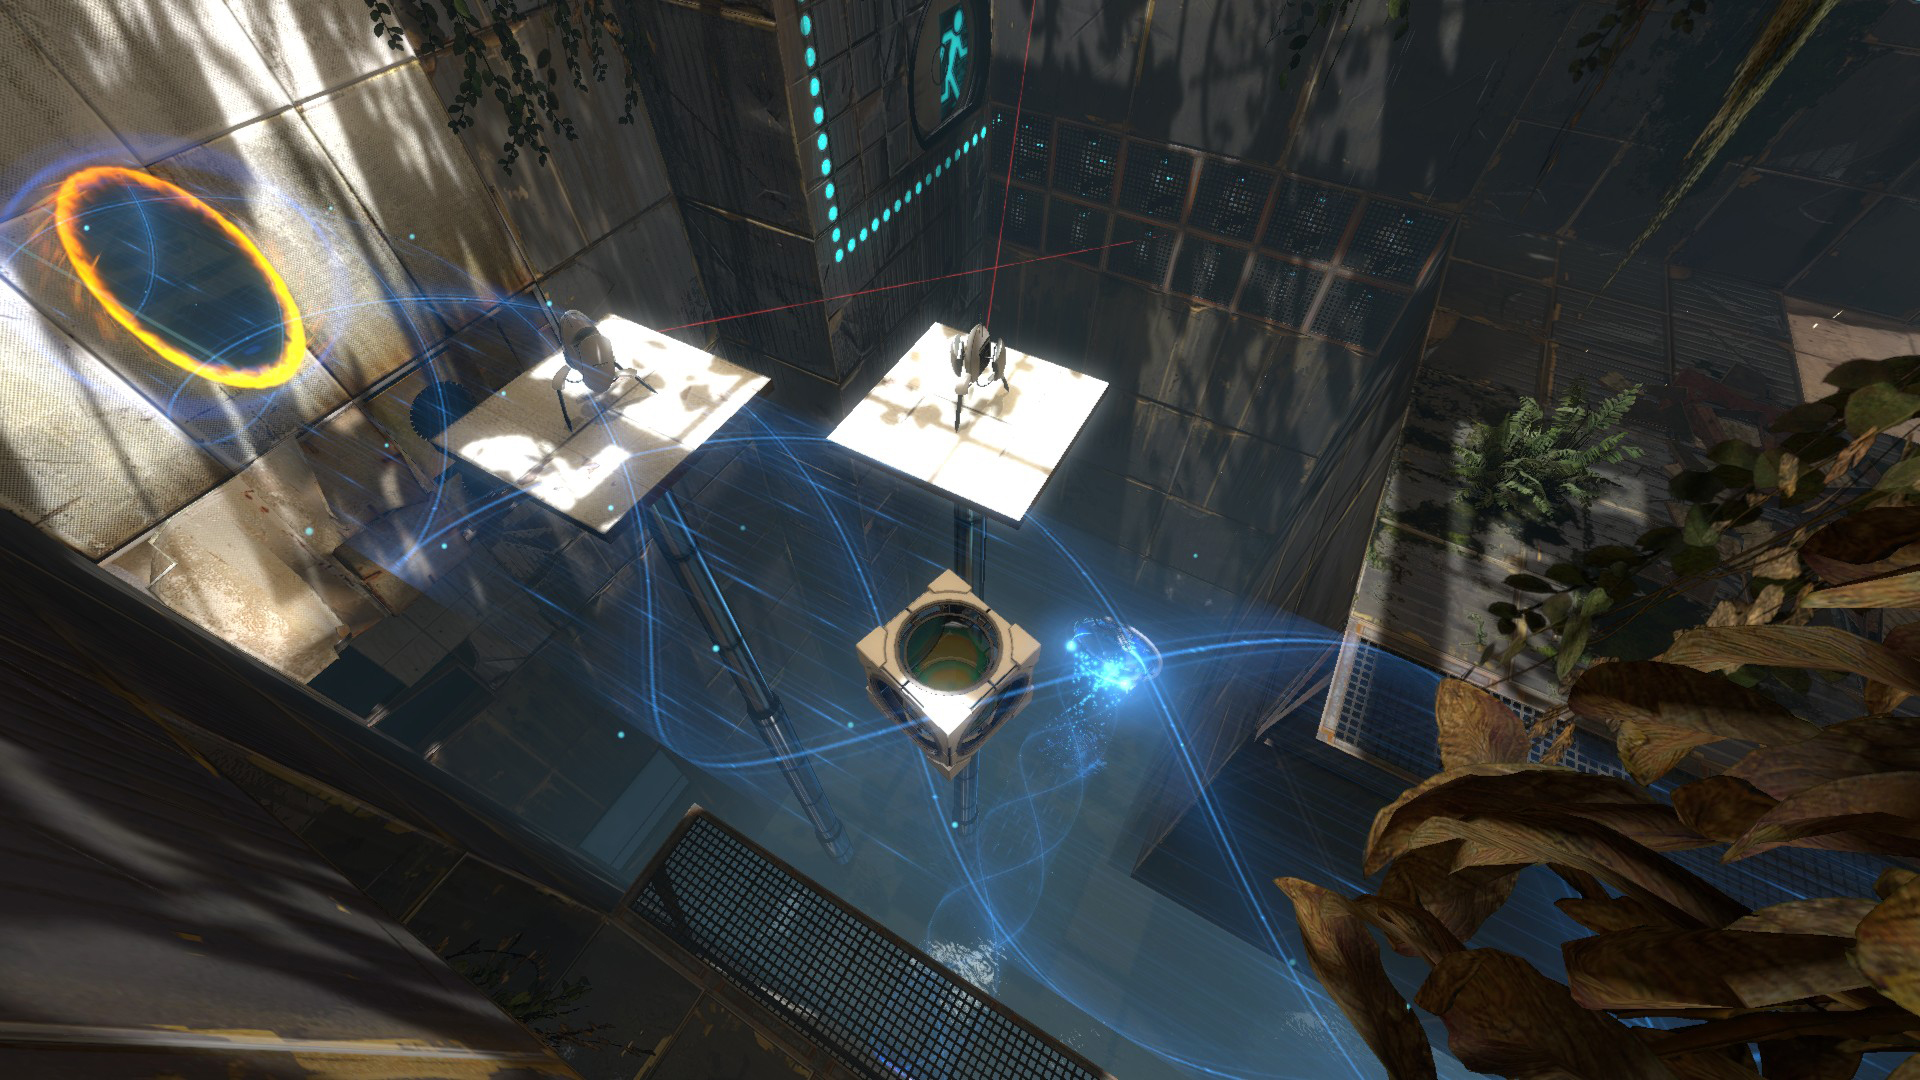
\includegraphics[width=0.8\textwidth]{portal2.jpg}
                \caption{Exemple de carte de Portal 2 utilisant une physique déformée (Les ondes bleues annulent la gravité et font dériver lentement dans leur direction)}
        \end{center}
        \end{figure}
        
        \begin{figure}[h]
        \begin{center}
            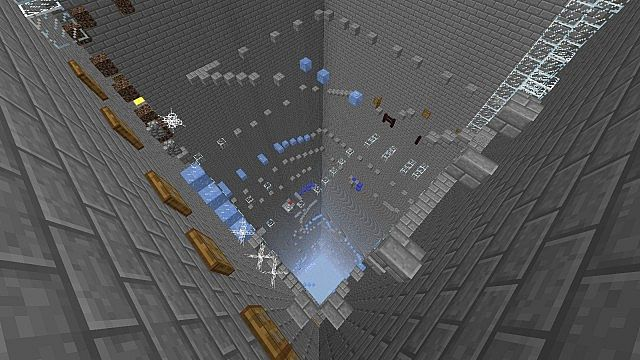
\includegraphics[width=0.8\textwidth]{minecraft.jpg}
                \caption{Exemple de carte "Parkour" de minecraft (Ici le joueur doit effectuer l'ascension d'une salle remplies de plate-formes de différents types)}
        \end{center}
        \end{figure}
        
        De plus nous pourrions nous considérer en concurrence avec les jeux à génération aléatoire de niveaux tels que le récent "No Man's Sky" présentant de la génération pseudo aléatoire d'écosystèmes.
        
    \subsection{Réalisation Logicielle}
        A la fin de ce projet seront disponibles deux produits partiellement indépendants. D'une part, un jeu avec un univers graphique complet accompagné d'une bibliothèque d'interaction et de décors prenant en entrée des descriptions de niveau et permettant d'y évoluer.
        Et d'une seconde part, un générateur de niveau qui utilisant une bibliothèque de décors et d'interactions génère aléatoirement la description d'un niveau jouable et agréable.
        
    \subsection{Organisation du projet}
        Nous avons décidé de nous séparer en deux sous équipes de 5. Une équipe pour s'occuper de la partie jeu (Loïs, Nicolas, Pierre, Pierre-Etienne, Yannis) et une autre équipe pour s'occuper de la partie générateur (Guillaume, Hugo, Rédouane, Thomas, Xavier).
        
        \begin{figure}[h]
        \begin{center}
            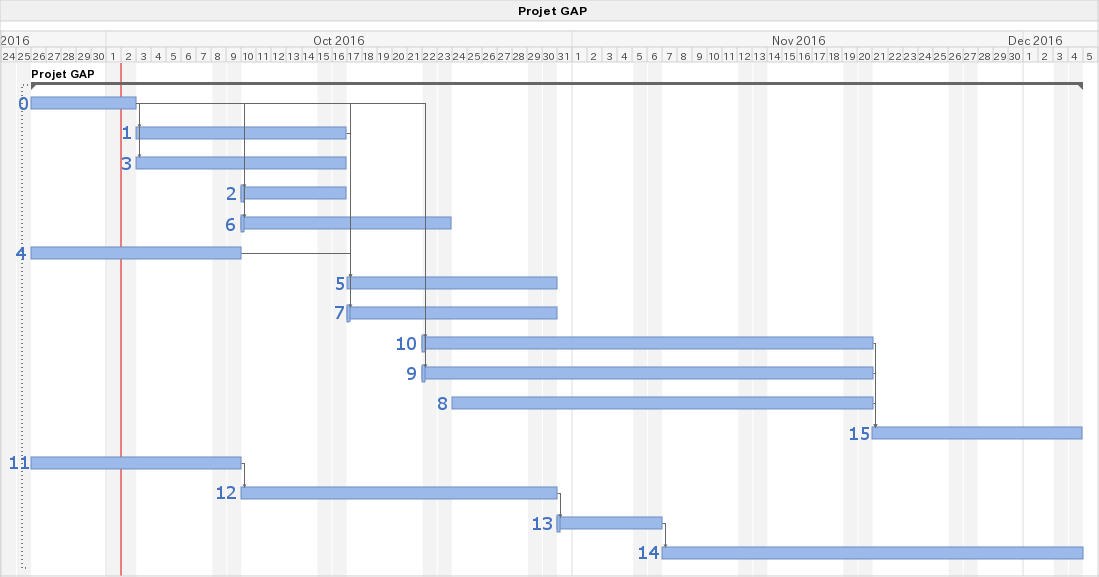
\includegraphics[width=1\textwidth]{gantt.png}
                \caption{Diagramme de Gantt prévisionnel du projet (Les dates de fin ne sont pas représentatives car l'on doit appliquer des semaines de pauses pour les partiels)}
        \end{center}
        \end{figure}
        
        Avec comme affectation des taches :
        \begin{enumerate}
            \setcounter{enumi}{-1}
            \item Apprentissage d'Unreal Engine 4 (Equipe jeu)
            \item \'Etudier les possibilités de 4D + tests comparatifs (Pierre, yannis)
            \item Créer l'interface utilisateur (menu, options, écran de jeu) (Yannis)
            \item \'Etudier les mécaniques de jeu réalisables (Nicolas, Pierre-Etienne, Loïs)
            \item Décider de la charte graphique + premier jet (Pierre)
            \item Intégrer l'interface utilisateur dans l'univers graphique du jeu (Pierre, Yannis)
            \item \'Etudier l'implentation des graphismes dans le moteur de jeu (Pierre, Nicolas)
            \item Définition du format de l'interface entre jeu et générateur (Nicolas, Yannis)
            \item Intégration des graphismes au jeu (Pierre, Nicolas)
            \item Design des plateformes et autres éléments de gameplay (Pierre-Etienne)
            \item Implémentation de la physique et des interactions (Loïs, Yannis)
            \item Définition du modèle
                \begin{itemize}
        \renewcommand{\labelitemi}{$\bullet$}
                    \item Qu'est-ce qu'un bon chemin de niveau (\'Equipe générateur)
                    \item Qu'est-ce qu'un bon sous niveau (Xavier, Guillaume)
                \end{itemize}
            \item Construction du niveau
                \begin{itemize}
        \renewcommand{\labelitemi}{$\bullet$}
                    \item Construction du chemin avec les zones d'influence (fixes puis dépendant des sous-niveaux) (Thomas, Hugo)
                    \item Construction des sous-niveaux (Xavier, Guillaume)
                \end{itemize}
            \item \'Evaluer le respect de la difficulté (\'Equipe générateur)
            \item Cycle tests et corrections du générateur (\'Equipe générateur)
            \item Cycle tests et corrections du jeu (\'Equipe jeu)
        \end{enumerate}
        
        \vspace{3mm}
        
        De plus nous avons nommés un certain nombres de responsables de sous parties:
        \begin{itemize}
        \renewcommand{\labelitemi}{$\bullet$}
            \item Pierre : Responsable Graphismes
            \item Hugo : Responsable Générateur
            \item Yannis : Responsable Jeu
            \item Loïs : Responsable Communication
        \end{itemize}
        
    \subsection{Financement}
    
        Dans un cadre où le financement serait disponible, nous envisageons de faire une application compatible Réalité Virtuelle, pour cela il nous faut le financement d'un casque de réalité virtuelle telle que l'HTC vibe ou bien l'oculus rift. L'oculus rift demanderais un budget de 699\euro et l'HTC vibe d'une qualité légèrement meilleure notamment du coté de l'affichage requiert un budget plus élevé de 899\euro.
\end{document}
